\documentclass{article}
\usepackage{amsmath}
\usepackage{graphicx}
\begin{document}

\title{On Collaborative Business Process Evolution}

\date{22-7-14}
\maketitle

\section{Introduction}
Companies merge with each other for many different reasons such as using each other's customers, and capacities in order to get a bigger market share.
The merge of companies can happen in many different forms depending on the lifeline of each of the companies after merge.
For instance, when a large company acquires a start-up, the start-up may be forced to follow the business processes (BPs) of the large company, since the it is not feasible, or even needed, to change the BPs of the large company to adapt to the ones of the start-up.

In the merge, which is the focus of this research, the two companies need to merge their BPs in order to achieve a common set of business process for using in the newly merged company.
In the merge process, each of the BPs of the two companies is either kept intact; discarded completely; or adapted to its corresponding business process in the other company.
The merge process is a collaborative process, since it needs the collaboration between the two companies, and, one the other hand, it is an iterative process not a one-pass process.
That is why we call it \emph{Collaborative Business Process Evolution} (CBPE in short), in this research.

  
The CBPE connotes two related concepts to the BP modeling. Firstly, the interactive concept  in BP modeling which is also surveyed as: "Group modeling", "Joint BP modeling", and "Collaborative BP design". The evolving characteristics is another concept in the CBPE. The evolution  indicates the capability of the changes in an information system, when a corresponding  BP evolves. Also, the evolution in BPs has a close meaning to  different term in BP modeling literature e.g. (re)design, improvement, re-engineering, and migration. 
However, there is not sufficient insight for collaboration in BP evolution (Niehaves and Henser, 2011) in the presented researches. Therefore, we aim at examining the collaborative business process evolution to introduce a supporting framework and evaluate it by case study.

\emph{•}
A number of challenging questions arise in merging the BPs of two companies.
As an example, consider the following questions:
\begin{itemize}
  \item It is better to design the BPs of the new company from scratch? or is it better to adapt the BPs of the two companies to the BPs of the new company? Which criteria can be used to choose between the two approaches?
  \item Which BPs should be kept, and which ones should be adapted?
  \item What\subsection{Collaborative [Business] Process Modeling/ Change/ Migration/ Redesign/ Re-engineering}
 parameters can be used in designing the new BPs?
  \item What roles in the companies are the best candidates for performing the merge process? and what authorities should they have?
  \item What is the best organizational structure for the groups who are responsible for performing the merge task?
  \item How the conflicts in rules, and the processes can be resolved?
  \item If the merge is done in a number of groups, what method should be followed in order to avoid or deal with the intra-group decisions that have side effects on the other groups?
  \item Is it possible that the newly merged BPs contain ambiguities while the original BPs, from which the merge BP is generated, do not contain ambiguity (for a definition of ambiguity refer to Section \ref{sec:pd}).
\end{itemize}

In this research, we aim at studying the CBPE problem.
As our test case, we use the currently ongoing merge of the science faculties of the University of Amsterdam (UvA), and the Vrije Universiteit (VU), which is part of a bigger plan for merging the two universities.

The rest of this report is structured as follows.
In Section \ref{sec:pd}, we define the notation, and standards which we use, precisely define the research questions that we aim to address, and further explain our test case.
In Section \ref{sec:approach}, we explain our approach for answering the research questions, and the metrics that we use to validate our research results.
Section \ref{sec:RW}, presents the related work.
In Section \ref{sec:tp}, we specify the detailed steps for this research together with the time plan.

\section{Problem Identification}\label{sec:pd}

\subsection{Background}
\subsubsection{BPMN}
BPMN 2.0 comprises more than one hundred elements, which are defined textually in the BPMN standards document. There is a depiction of the main BPMN 2.0 elements  \cite{Bpmn13} in Fig.\ref{fig:figure1}. They can be represented in six categories. "Events", "Activities",  "Gateways", "Connectivity objects", "Swimlanes", and "Artifacts". 

\begin{figure}
\centering%
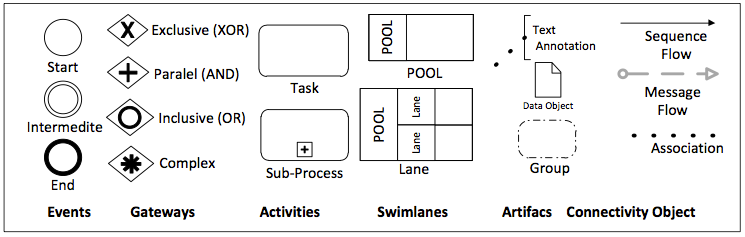
\includegraphics[scale=0.45]{BPMN_Symbols.png}
\caption{BPMN 2.0 Basic Elements} 
\label{fig:figure1}
\end{figure}

The three first categories describe the sequence of different BPMN elements in a business flow. An \textit{event} represents an occurrence which happens during the business process and has an interaction with the environment. Regarding proactive and reactive roles of \textit{events}, they affect the flow of the process and  have a cause(trigger) or an impact(result). The main types of \textit{events} include: \textit{Start}, \textit{Intermediate} and \textit{End}.

\textit{Activities} include tasks or (sub)processes of an enterprise, which represent a specific break of the work. They can be atomic or non-atomic tasks. Processes and sub-processes can be defined in more detail, while tasks can not be broken down further.

\textit{Gateways} are used to define the types of control behaviors of  BP flows. They capture  branching, forking, merging and joining of the flow threads. Some are as follows:
\textit{Exclusive gateways} makes substitution path in process flow and describe a behavior, which is equal to the XOR logical concept. 
\textit{Inclusive gateway} decision making is about the behavior of alternative or parallel paths in process flow and is similar to OR concept.
\textit{Parallel gateway} either in forking or joining situation, represents the synchronization in execution of activities. its concept is close to AND.
Complex gateway is for complex decisions, i.e. selecting "n" out of "m" possible existing alternatives.. 

Generally speaking, \textit{Connectivity objects} represent the three main flow streams in BP activities. \textit{Sequence flows} show the execution order of activities. The direction of exchanged messages are shown by \textit{message flows}. The directed interactions of parties and participants in a BPD are depicted by \textit{associations} link.

\textit{Swimlanes} include Lanes and Pools. \textit{Lanes} are the basis of flows usually for a participants and business context, while \textit{pools} cover interactions and collaborations of different participants. 

\textit{Artifacts} in BPMN imply in explanations in three different forms.\textit{ Data objects} cover the informational aspect of business execution in parallel with control flow. The common context of a set of activities is depicted by \textit{group} symbol. Extra explanations for user and further readability of BPDs are available by using \textit{text annotations} in BPMN models.
\subsubsection{Ambiguity}
Through surveying the suitability of different BP modeling languages and standards, BPMN (ver. 2.0) is introduced as the proper candidate for BP formalizing and behavior capturing. Its executable semantics and rich syntax help business analysts and domain experts in modeling the real-world systems. However, there are some deficiencies and ambiguities in BPMN depiction and execution. Some of them is represented as follows.
There are some BPMN has the missing the general notion of state as the sequence of activity. It emerges because of the chosen level of abstraction for keeping the understandability of graphs versus having extra level of detail. “Resource” in Business process modeling is an entity, which is responsible for doing a work. It could be a human, (e.g. employee of an organization) or non-human (a machine in factory). The resources have their levels and hierarchy in an organization or other contexts. They may have delegate, which means temporarily change in responsibility (for example of a human actor). Moreover, they could have roles, which address a category of similar responsibility of human actors. Non-human resources may have capability of consumption or history of work. In BPMN the only mechanism, which partially supports resource management is lanes.
BPMN standard does not restrict modeler to a specific methodology in diagramming. Thus, different types of diagrams eliminate (de) composition of BPDs, especially in case of arbitrary cycles. There is a poor support of concurrent and synchronized structures, especially for execution purposes. For example OR-join notion or other synchronized methods. BPMN execution is hard to achieve. That is because of the lack of seamless mechanism in its standard draft. This issue forces using mediated languages (i.e. BPEL) in execution phase. However, this leads to syntactic mismatches (because of different intrinsic of languages) or difficulties in understandability (because of using textual notation instead of graphical depiction). Although, the BPMN standard endeavors to make a unified comprehension, but there are example of different understands from same diagrams or different execution complied from same construct (e.g. BPMN -2-BPEL and BPEL-2- BPMN)  
These deficiencies and ambiguities are categorized in two-folds: “Intrinsic” and “Utilization”. The intrinsic ambiguities originally exist in BPMN syntax, and difficult to eliminate (e.g. OR-join or event based gateway syntax). The utilization ambiguities refer to the specific patterns, which completely (e.g. Milestone) or partially ( e.g. structured discrimination) are not supported by BPMN.
Therefore, for precise and concise execution, an unambiguous BPMN depiction is needed. Moreover, it is necessary to include the mistake or limitation of the system analysts in providing BPMN Diagrams. Thus, we deal with ambiguities either by replacing the pattern with unambiguous pattern, or by adding notations to BPMN to enable high level support of the pattern, if required. Furthermore, we detect possible misuse of the patterns and suggest possible correction to the user (for generating robust code).

 \subsection{Example}
 The University of Amsterdam (UVA) and the VU University of Amsterdam (VU) have decided to form an alliance between their faculties of science. This alliance includes inter- and intra- organizational changes in goals, policies, and specifically routines in form of a new organization, so called Amsterdam Faculty of Science (AFS). In other word, the UVA and VU are unifying their academical affairs (e.g. teaching) and supporting activities (e.g. human resource activity). Therefore, they need to collaborate for evolving their Business Processes (BPs) e.g. hiring a new employee, or employing a PhD student.
% Employment hiring example is inserted here
 The BP modeling and changing efforts are part of organizations job, while collaboration and the collaborative process of evolving make it challenging.
 
  alliance of  VU and UVA
 exemplify of  a common BP (HR)
 collaboration for BP evolution
 collaboration for achieving unambiguous BP
 \subsection{Research Questions}
 RQs list
 Outcomes
 Assumptions

\section{Research Approach}\label{sec:approach}

Research approach for the first part
Research approach for the second part
Solution
Metrics and validation 

\section{Related work}\label{sec:RW}
\subsection{BP/Collaborative BP}

\subsection{Group [Business]  Process Modeling/ Change/ Migration/ Redesign/ Re-engineering}\label{GM)}
In 90s, the concept of “group modeling” and “group business process modeling” surveyed different aspects of tools, systems, and number of contributors, to achieve more efficiency, better quality and faster results (Dean et al. 1994).


\subsection{Collaborative [Business] Process Modeling/ Change/ Migration/ Redesign/ Re-engineering}
 
 \subsection{Joint [Business] Process Modeling/ Change/ Migration/ Redesign/ Re-engineering}

 \subsection{Collaborative [Business] Process merge/ Integration}

To elaborate a conceptual model for designing a particular information system, a visual representation by a set of specific artifacts from a distinguished context is needed (Wand and Weber, 2002). The BP model is a conceptual model, whereas it captures the external behavior of a process. Moreover, BP modeling is performed by languages, which consist of grammars and semantics (e.g. BPMN, UML) (Riemer et.al, 2011). Beside model and modeling languages, the modeler is another part of system design, and usually includes a group of stakeholders.

The modeling could be accomplished by domain experts, consultants (Xiao and Zheng, 2012), facilitators (Hengst, 2005), and editing tools (Rittgen, 2010). The joint modelling to make a shared understanding of models, so-called collaborative modelling has been live topic for two recent decades ( Renger et al., 2008).  It was a source of many empirical experiments and case studies. 

A number of researches focus on knowledge transmission during modelling (Xiao and Zheng, 2010). Renger et al. introduced a number of issues for collaborative modelling, i.e., group composition trade-offs between stakeholders and domain experts, or choose of starting point for modelling either from experts creation or from domain experts’ scratchs. 

A series of extensive research for collaborative modelling is presented by Rittgen. He presents a negation model for recognizing different levels and domain of the collaborative modelling in social, pragmatic, and language aspects (Rittgen, 2007). Also, a model of collaborative factors is elaborated in (Rettgen, 2010b), which addresses the co-evolution of methods and tools towards increasing group productivity.  Other collaborative modelling researches focus on supporting software infrastructure (Hahn et al., 2011) or collaboration facilitator tools ( Riemer et al. 2011).

However, there is not sufficient insight for collaboration in BP evolution (Niehaves and Henser, 2011) in the presented researches. Therefore, we aim at examining the collaborative business process evolution to introduce a supporting framework and evaluate it by case study.


\section{Time plan}\label{sec:tp}



\section{refrence}\label{ref}
 OMGGroup: Business process model and notaion (bpmn) version 2.0.2 (Dec 2013)
Dean, D. L., Lee, J. D., Orwig, R. E., and Vogel, D. R. (1994). Technological support for group process modeling. Journal of Management Information Systems, 43-63.


Dumas, M., La Rosa, M., Mendling, J., and Reijers, H. A. (2013). Fundamentals of business process management (pp. I-XXVII). Heidelberg: Springer.


Dijkman, R. M., Dumas, M., and Ouyang, C. (2008). Semantics and analysis of business process models in BPMN. Information and Software Technology, 50(12), 1281-1294.


Hahn, C., Recker, J., and Mendling, J. (2011, January). An exploratory study of IT-enabled collaborative process modeling. In Business Process Management Workshops (pp. 61-72). Springer Berlin Heidelberg.


Hengst, M. D. (2005). Collaborative Modeling of Processes: What Facilitation Support Does a Group Need?. AMCIS 2005 Proceedings, 15.


Niehaves, B., and Henser, J. (2011). Boundary spanning practices in BPM: a dynamic capability perspective.
Renger, M., Kolfschoten, G. L., and de Vreede, G. J. (2008). Challenges in collaborative modeling: A literature review. In Advances in Enterprise Engineering I (pp. 61-77). Springer Berlin Heidelberg.

Riemer, K., Holler, J., and Indulska, M. (2011). Collaborative process modelling-tool analysis and design implications.


Rittgen, P. (2007, January). Negotiating models. In Advanced information systems engineering (pp. 561-573). Springer Berlin Heidelberg.


Rittgen, P. (2010). 19P. Collaborative Business Process Modeling–Tool Support for Solving Typical Problems.


Rittgen, P. (2010,b). Success factors of e-collaboration in business process modeling. In Advanced Information Systems Engineering (pp. 24-37). Springer Berlin Heidelberg.


Russell, N., Ter Hofstede, A. H., and Mulyar, N. (2006). Workflow controlflow patterns: A revised view.


Xiao, L., and  Zheng, L. (2012). Business process design: Process comparison and integration. Information Systems Frontiers, 14(2), 363-374.


Wand, Y., and Weber, R. (2002). Research commentary: information systems and conceptual modeling—a research agenda. Information Systems Research, 13(4), 363-376.



























\end{document} 